\subsection{UAV Toolbox}
To achieve a visual way for checking if the quadrotor plant has been constructed correctly, the UAV Toolbox was used. (See Figure \ref{fig:3dsimulation})
For studying PID control, the MATLAB UAV 3D simulation provides a realistic and interactive environment.
The simulation was used to examine the behavior of the UAV system rather than relying exclusively on theoretical concepts and mathematical equations. 
Experiments with different PID controller parameters were conducted, to see how they affect the quadrotor's reaction and acquire hands-on experience tweaking the controller. This immersive learning experience aid in the integration of theory and practice.
Control performance in complex circumstances can be analyzed using the MATLAB UAV 3D simulation. When numerous PIDs are involved, it can become difficult to intuitively understand how one effects another; thus, a visual representation aids in grasping and understanding the concepts.
\begin{figure}[H]
    \begin{center}
    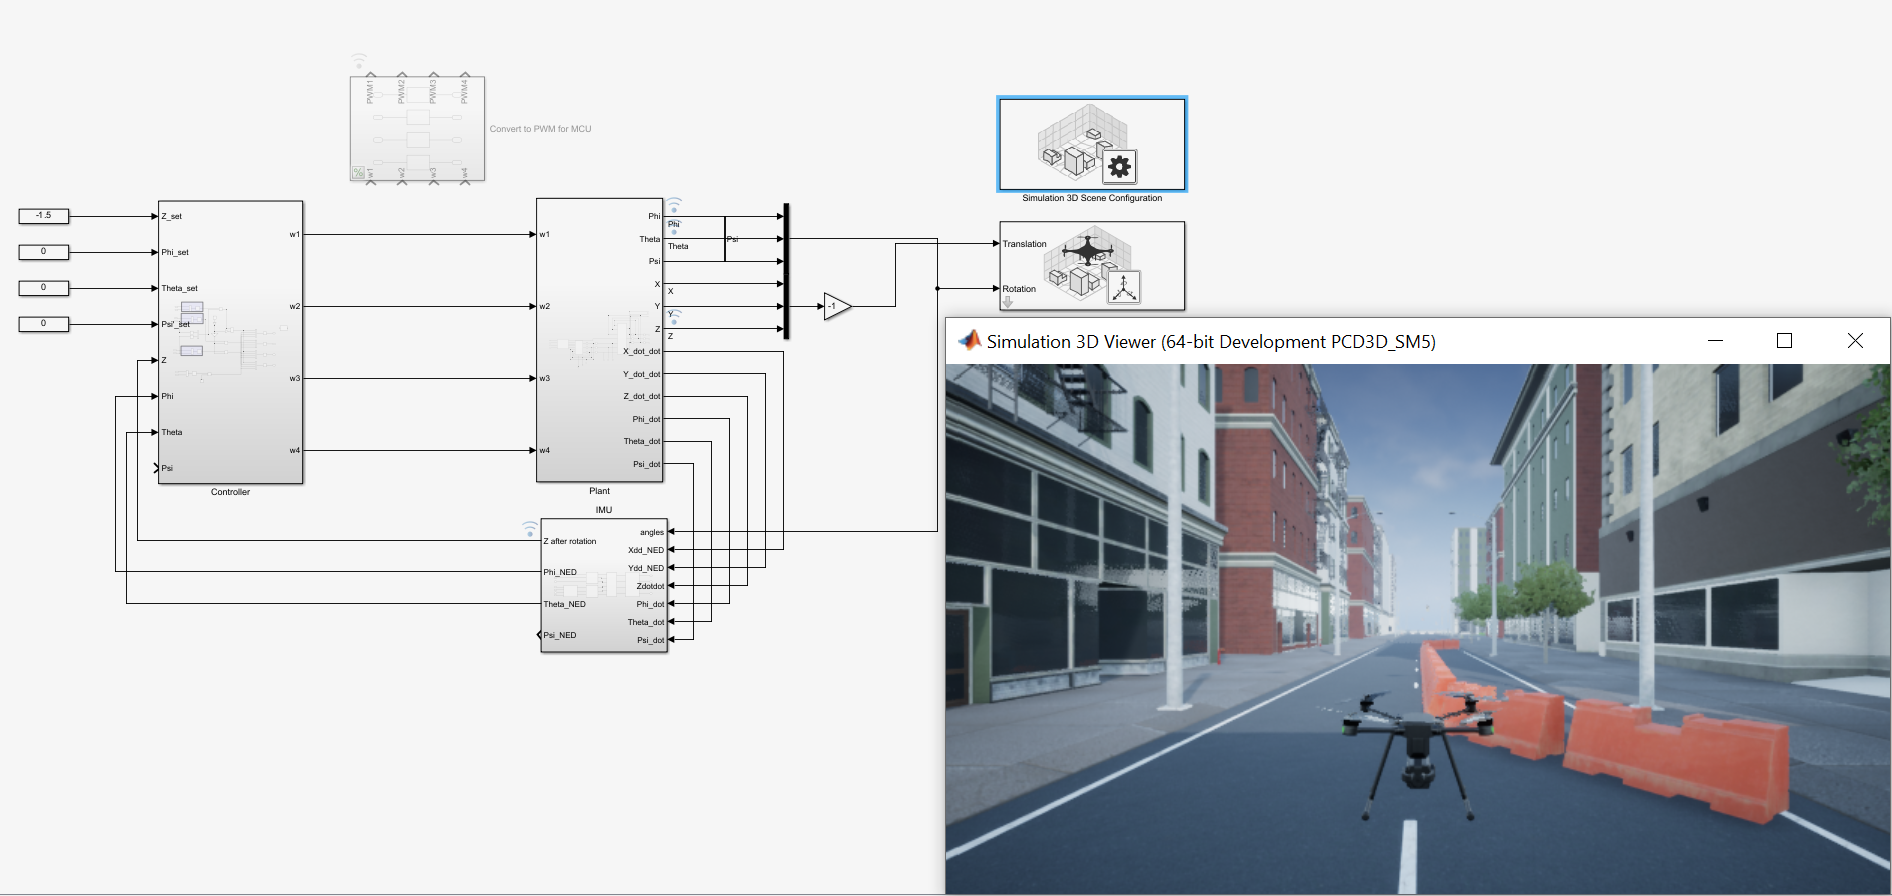
\includegraphics[scale=0.4]{pictures/control/3dsimulation}
    \end{center}
    \caption{Ilustration of the workflow, with the utilization of the UAV Toolbox}
    \label{fig:3dsimulation}
\end{figure}